\documentclass[twocolumn,landscape,8pt]{article}
\usepackage{lipsum}% http://ctan.org/pkg/lipsum
\usepackage{graphicx,dblfloatfix}% http://ctan.org/pkg/{graphicx,dblfloatfix}
\usepackage{longtable}
\usepackage{tikz}
\usepackage{blindtext}
\usepackage{calendar} % Use the calendar.sty style
\usepackage[condensed,math]{anttor}
\usepackage[T1]{fontenc}
\usepackage{pdfpages}


\usepackage[landscape,margin=0.5in]{geometry}
\newcommand\framethispage[1][1cm]{%
    \tikz[overlay,remember picture,line width=1pt]
    \draw([xshift=(#1),yshift=(-#1)]current page.north west)rectangle
         ([xshift=(-#1),yshift=(#1)]current page.south east);%
}

\usepackage{catchfile}
\newcommand{\getenv}[2][]{%
  \CatchFileEdef{\temp}{"|kpsewhich --var-value #2"}{}%
  \if\relax\detokenize{#1}\relax\temp\else\let#1\temp\fi}

\begin{document}
\framethispage[0.2cm]% le cadre est à 2 cm des bords de la feuille

\getenv[\RES]{RES}\show\RES

\title{Finance}

%Example de la police que je voulais

\makeatletter
\newcommand\CTFont[1][small]{
\renewenvironment{table}
               {\@float{table}\csname#1\endcsname}
               {\end@float}
\renewenvironment{table*}
               {\@dblfloat{table}\csname#1\endcsname}
               {\end@dblfloat}
}
\makeatother

\maketitle

%\blindtext
%    \begin{tikzpicture}[remember picture,overlay]
%    \node[anchor=north west,yshift=-15pt,xshift=15pt]%
%        at (current page.north west)
%        {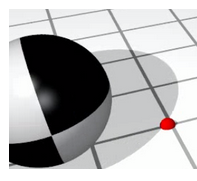
\includegraphics[height=15mm]{Logo}};
%    \end{tikzpicture}
%\blindtext

%{\footnotesize
%Blalalallalalal/home/frederickerdraon/Documents/researchwork/Latex/
%}

%\begin{figure*}[b]
%  \centering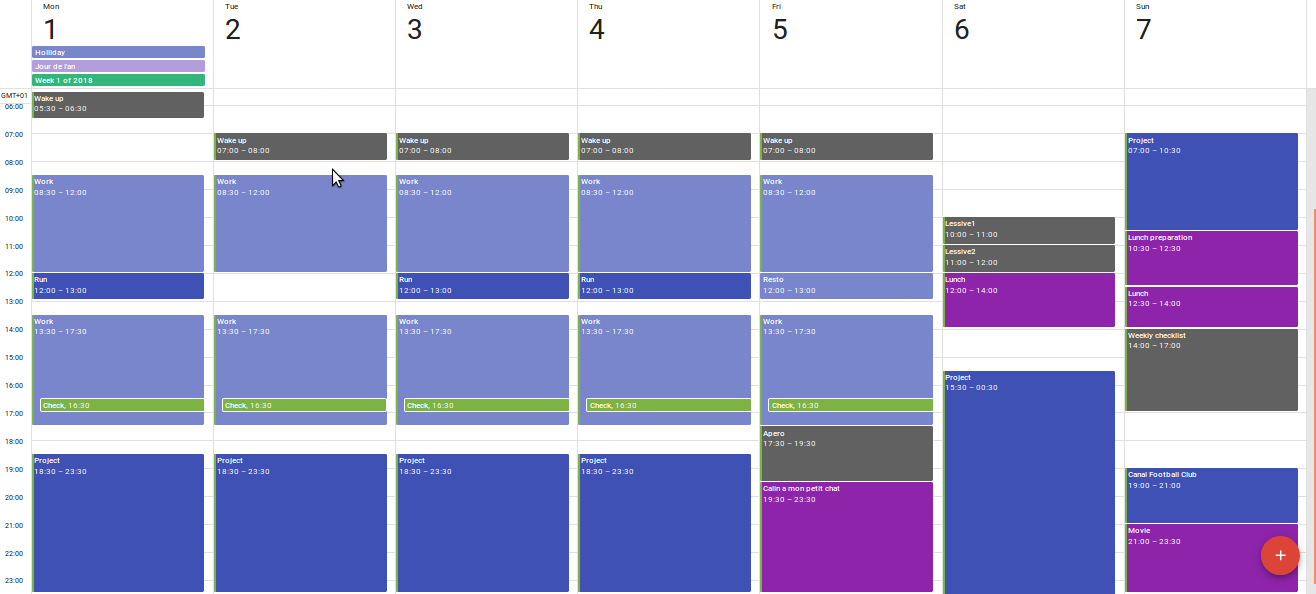
\includegraphics[width=\linewidth,height=0.3\textheight]{cal1}
%  \caption{B caption}
%\end{figure*}

%\begin{figure*}[t]
%  \centering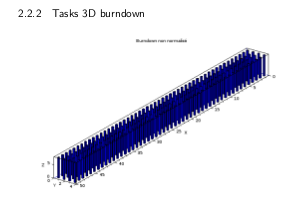
\includegraphics[width=\linewidth,height=0.3\textheight]{burn}
%  \caption{B caption}
%\end{figure*}

%\lipsum[4-7]

\begin{figure}[t]
  \centering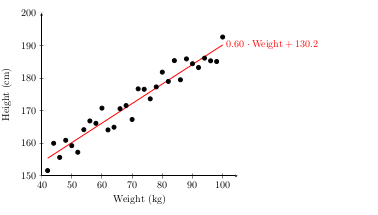
\includegraphics[width=\columnwidth,height=0.1\textheight]{linear}
  %\caption{A caption}
\end{figure}

%{\footnotesize
%Blalalallalalal
%}

%Mon texte de base ici
\begin{figure}[t]
  \centering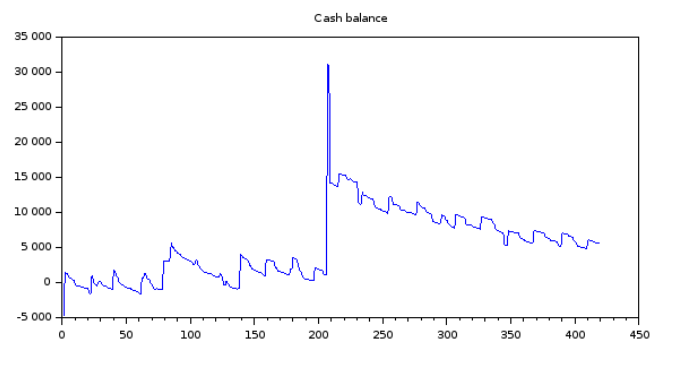
\includegraphics[width=\columnwidth,height=0.2\textheight]{cash}
  %\caption{A caption}
\end{figure}

\begingroup
%\CTFont% tables in \small size
\CTFont[tiny]% tables in \tiny size
\begin{figure}[t]
{\footnotesize
\input{$RES/Latex/cashflows}
}
\end{figure}
\endgroup

\begin{figure}[t]
{\footnotesize
\input{/home/frederickerdraon/Documents/researchwork/Latex/contacts}
}
\end{figure}

\begin{figure}[t]
  \centering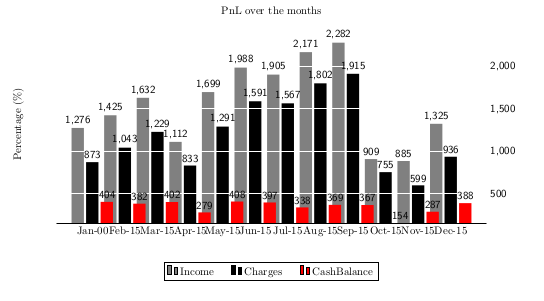
\includegraphics[width=\columnwidth,height=0.3\textheight]{pnl}
  %\caption{A caption}
\end{figure}

%\begin{figure}[t]
%  \centering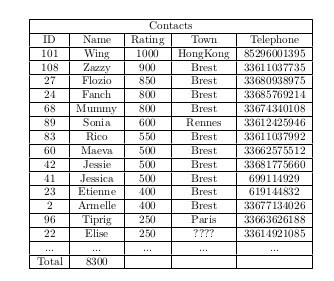
\includegraphics[width=\columnwidth,height=0.3\textheight]{contacts}
  %\caption{A caption}
%\end{figure}

%\begin{figure}[t]
%  \centering\includegraphics[width=\columnwidth,height=0.3\textheight]{tasks}
  %\caption{A caption}
%\end{figure}

\begin{figure}[t]
{\footnotesize
\input{/home/frederickerdraon/Documents/researchwork/Latex/tasks}
}
\end{figure}

%\begin{figure}[t]
%{\footnotesize
%\input{/home/frederic/researchwork/MyFirstWindow/Latex/events}
%}
%\end{figure}

%\begin{figure}[t]
%{\footnotesize
%\input{/home/frederic/researchwork/MyFirstWindow/Latex/chargesCheese}
%}
%\end{figure}

%\begin{figure}[t]
%  \centering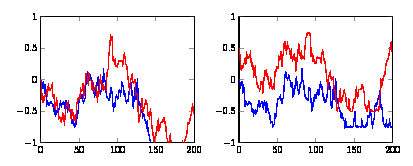
\includegraphics[width=\columnwidth,height=0.1\textheight]{Brownian}
%  \caption{A caption}
%\end{figure}
%Tentative 
\begin{figure}[t]
  \centering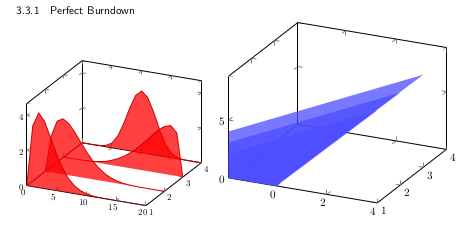
\includegraphics[width=\columnwidth,height=0.1\textheight]{burndown}
  %\caption{A caption}
%

\documentclass[border=10pt]{standalone}
\usepackage{pgfplots}
\pgfplotsset{width=7cm,compat=1.8}
\usepackage{pgfplotstable}
\renewcommand*{\familydefault}{\sfdefault}
\usepackage{sfmath}
\begin{document}
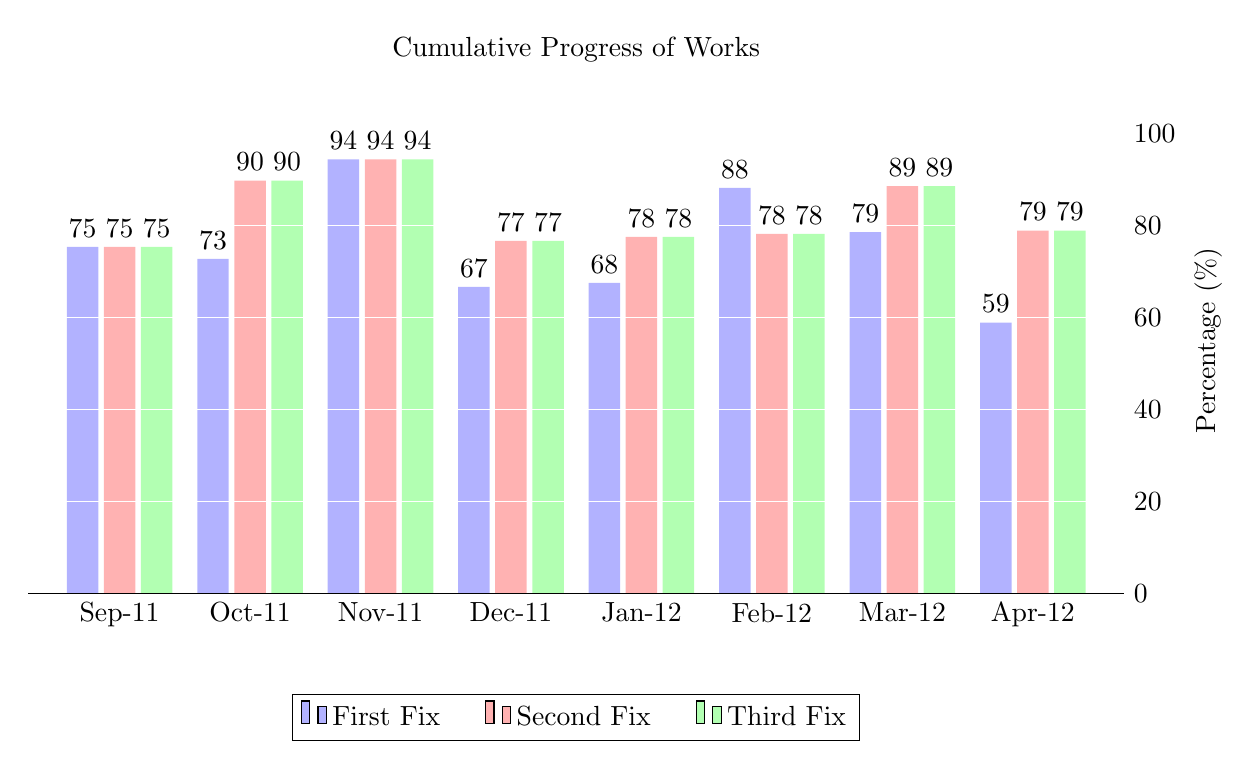
\begin{tikzpicture}
  \centering
  \begin{axis}[
        ybar, axis on top,
        title={Cumulative Progress of Works},
        height=8cm, width=15.5cm,
        bar width=0.4cm,
        ymajorgrids, tick align=inside,
        major grid style={draw=white},
        enlarge y limits={value=.1,upper},
        ymin=0, ymax=100,
        axis x line*=bottom,
        axis y line*=right,
        y axis line style={opacity=0},
        tickwidth=0pt,
        enlarge x limits=true,
        legend style={
            at={(0.5,-0.2)},
            anchor=north,
            legend columns=-1,
            /tikz/every even column/.append style={column sep=0.5cm}
        },
        ylabel={Percentage (\%)},
        symbolic x coords={
           Sep-11,Oct-11,Nov-11,Dec-11,
           Jan-12,Feb-12,
           Mar-12,
          Apr-12},
       xtick=data,
       nodes near coords={
        \pgfmathprintnumber[precision=0]{\pgfplotspointmeta}
       }
    ]
    \addplot [draw=none, fill=blue!30] coordinates {
      (Sep-11,75.4064)
      (Oct-11, 72.7961) 
      (Nov-11,94.4597)
      (Dec-11,66.6786) 
      (Jan-12,67.5600) 
      (Feb-12,88.2339)
      (Mar-12,78.6138) 
      (Apr-12,58.9129) };
   \addplot [draw=none,fill=red!30] coordinates {
      (Sep-11,75.4064)
      (Oct-11, 89.7961) 
      (Nov-11,94.4597)
      (Dec-11,76.6786) 
      (Jan-12,77.5600) 
      (Feb-12,78.2339)
      (Mar-12,88.6138) 
      (Apr-12,78.9129) };
   \addplot [draw=none, fill=green!30] coordinates {
      (Sep-11,75.4064)
      (Oct-11, 89.7961) 
      (Nov-11,94.4597)
      (Dec-11,76.6786) 
      (Jan-12,77.5600) 
      (Feb-12,78.2339)
      (Mar-12,88.6138) 
      (Apr-12,78.9129) };

    \legend{First Fix,Second Fix,Third Fix}
  \end{axis}
  \end{tikzpicture}
\end{document}


\end{figure}

%\begin{figure*}[b]
%  \centering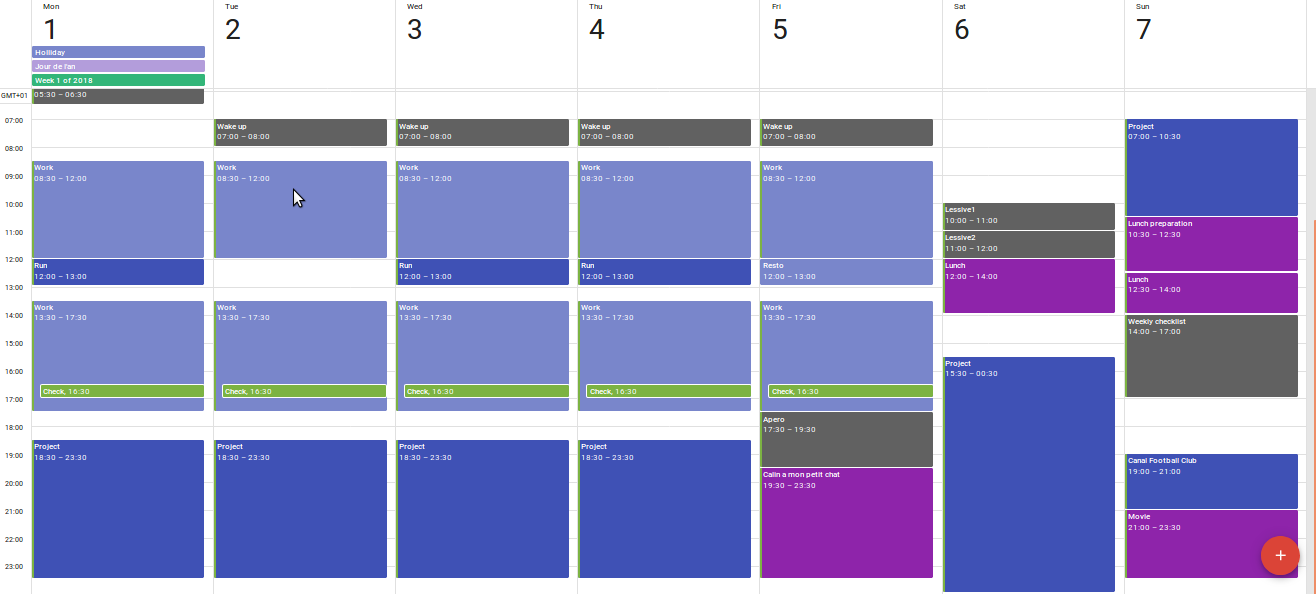
\includegraphics[width=\linewidth,height=0.6\textheight]{cal}
%  %\caption{B caption}
%\end{figure*}

%\begin{figure}[t]
%{\footnotesize
%\input{/home/frederic/researchwork/MyFirstWindow/Latex/calendar_3}
%}
%\end{figure}


\begin{figure}[t]
  \centering\includegraphics[width=\columnwidth,height=0.1\textheight]{/home/frederic/researchwork/MyFirstWindow/Latex/tasks}
  \caption{A caption}
\end{figure}

\begin{figure}[t]
{\footnotesize
  \input{/home/frederickerdraon/Documents/researchwork/Latex/cashflows_other}
}
\end{figure}

% Ici on change pour ne mettre les éléments que sur une seule colonne, c'est à dire la page complète
% Ici on change pour ne mettre les éléments que sur une seule colonne, c'est à dire la page complète
\begingroup
\onecolumn
\begin{figure}[t]
  \centering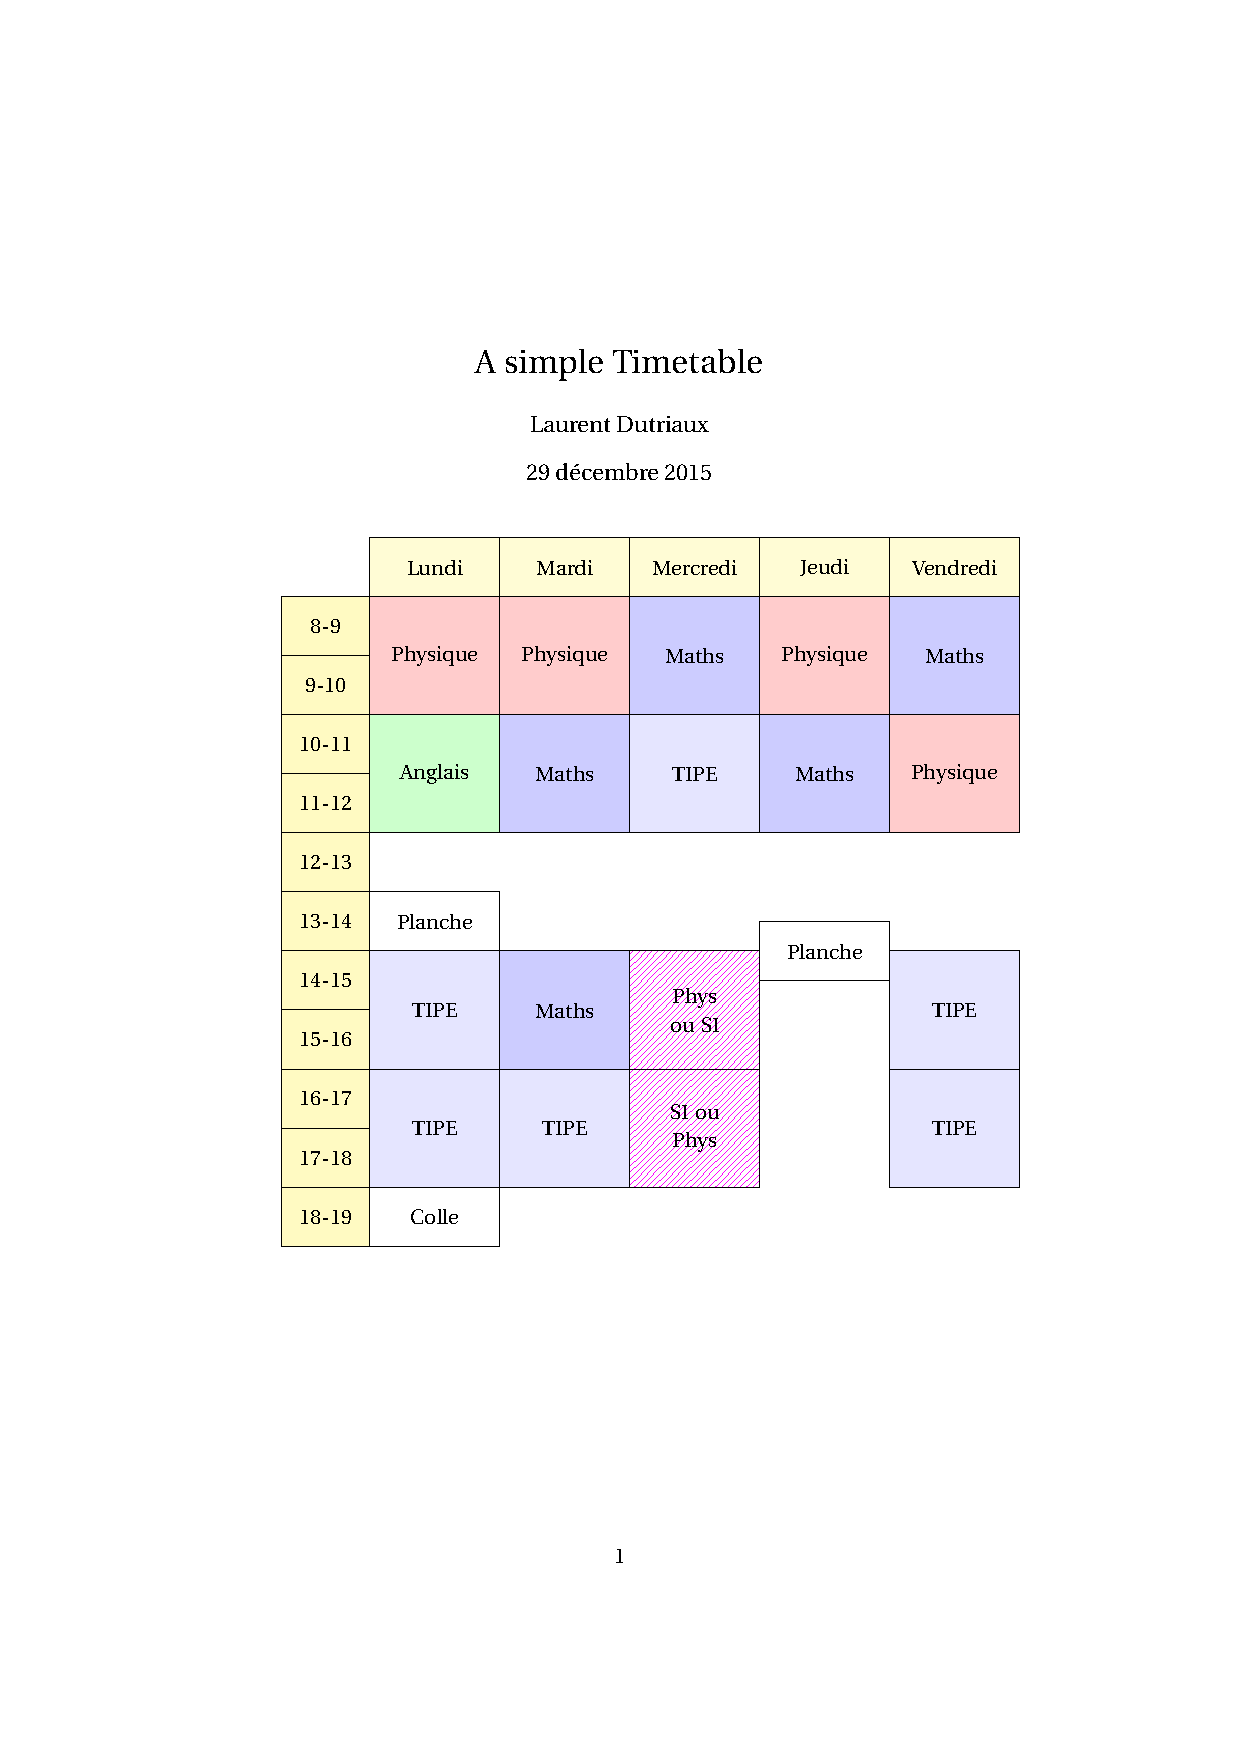
\includegraphics[width=\columnwidth,height=1.0\textheight]{TimeTable}
  \caption{A caption}
\end{figure}
\endgroup

\begingroup
\onecolumn
\begin{figure}[t]
\includepdf[pages={1}]{/home/frederickerdraon/researchwork/Latex/Calendar17.pdf}
\end{figure}
\endgroup

%\onecolumn
%\begingroup
%\centering
%{\LARGE The Title \\[1.5em]
%\large First Author\Mark{1}, Second Author\Mark{2}, Third Author\Mark{1}, Fourth Author\Mark{2} and Fifth Author\Mark{3}}\\[1em]
%\begin{tabular}{*{2}{>{\centering}p{.25\textwidth}}}
%\Mark{1}Department1 & \Mark{2}Department2 \tabularnewline
%School1 & School2  \tabularnewline
%\url{email1} & \url{email2}
%\end{tabular}\par
%\twocolumn
%\endgroup

%\begin{figure}[t]
%  \centering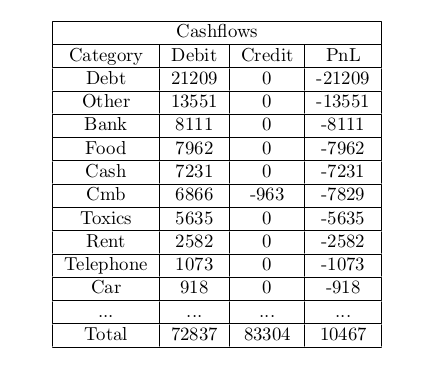
\includegraphics[width=\columnwidth,height=0.1\textheight]{expenses}
  %\caption{A caption}
%\end{figure}

%\lipsum[8-12]
\end{document}
